\documentclass[a4paper,12pt,twoside]{article}

\usepackage[utf8]{inputenc}
\usepackage[T2A]{fontenc}
\usepackage[english]{babel}
\usepackage{booktabs}
\usepackage[margin = 1in,includeheadfoot]{geometry}
\usepackage{graphicx}
\usepackage{amsmath}
\usepackage{amssymb}
\usepackage{tikz}
\usepackage{fancyhdr}

\parindent=0pt
\parskip=10pt

\pagestyle{fancy}
\fancyhf{}
\rhead{Sasha Petrov}
\lhead{}
\rfoot{\thepage}
\setlength{\headheight}{14.5pt}

%hyperlinks package -- should be the last to import
\usepackage{hyperref}
\hypersetup{
	colorlinks = true,
	linkcolor=blue,
	citecolor=blue,
	urlcolor=blue }
	
\title{ECON 31703: Assignment 1}
\author{Sasha Petrov}

\usepackage{Sweave}
\begin{document}
\Sconcordance{concordance:ps1.tex:ps1.Rnw:%
1 34 1 1 0 12 1 1 5 4 0 1 3 17 1 1 3 12 0 1 3 4 1 1 3 12 0 1 3 19 1 1 3 %
29 0 1 3 30 1 1 3 1 0 4 1 1 2 14 0 1 2 49 1 1 3 38 0 1 3 1 1}


\maketitle


\section*{Exercise 1}


\subsection*{(b)}

Here are the empirical mean and variance of the estimator that only uses one regressor:

\begin{Schunk}
\begin{Soutput}
[1] 1.00177040 0.02037899
\end{Soutput}
\end{Schunk}


\subsection*{(c)}

The output is reported below: columns are different choices of $\tilde p$, 1st row -- mean of $\hat\beta_1$, 2nd row -- variance.

2 observations about the table:

\begin{itemize}
  \item For any choice of $\tilde p$ the estimate `targets' the true value of $\beta_1$ pretty well -- which is not surpising given that covariates are orthogonal, so there's no confounding going on.
  \item The variance of the estimate increases with $\tilde p$; I see 2 possible explanations for this (both of which come from looking at the asymptotic approximation for the variance of $\hat \beta_1$: $\sigma \mathbb{E} \left[ \mathbf{X} \mathbf{X}' \right]^{-1}$; the problem with this approach is that this asymptotic approximation is the same regardless of $\tilde p$; due to that, I'll cheat and assume that the estimation process of this variance reflects difficulties/imprecision in the asymptotic approximation -- btw very curious if this approach has any real/heuristic ground in theory):
  \begin{itemize}
    \item We need to calculate the inverse of the matrix that's approximately an identity matrix $\frac{1}{N} \sum_{i = 1}^N \mathbf{X}_i \mathbf{X}'_i$; my guess: as the dimensions increase the inverse will `move further' from the identity matrix (which should be the result in theory), probably due to computational difficulties;
    \item We need to estimate the variance of the error $\sigma$ which is connected to a) how well the model is fit; b) the number of regressors. My guess: because regressors are orthogonal, the decrease in the variance of prediction errors is modest with an increase in $\tilde p$; while the correction for the number of regressors kicks in significantly and mechanically increases the variance.
  \end{itemize}
\end{itemize}


\begin{Schunk}
\begin{Sinput}
> print(table_c)
\end{Sinput}
\begin{Soutput}
           [,1]       [,2]       [,3]       [,4]      [,5]
[1,] 1.00073173 1.00089195 1.00252512 1.00130035 1.0026628
[2,] 0.01065004 0.01129519 0.02012384 0.07253589 0.1125315
\end{Soutput}
\begin{Sinput}
> 
\end{Sinput}
\end{Schunk}


\subsection*{(d)}


\begin{Schunk}
\begin{Sinput}
> print(table_d)
\end{Sinput}
\begin{Soutput}
           [,1]       [,2]      [,3]        [,4]        [,5]
[1,] 0.74002279 0.55677025 0.1049905 0.009696993 0.004918019
[2,] 0.03999503 0.09021956 0.4907584 0.842317676 0.892350986
\end{Soutput}
\begin{Sinput}
> 
\end{Sinput}
\end{Schunk}

\textit{How to read the table:} columns -- different choices of $\tilde p$;
row 1 -- lower eigenvalue; row 2 -- average squared prediction.


Two observations:

\begin{itemize}
  \item The estmated lowest eigenvalue decreases significantly as $p$ increases. 
  This probably reflects the empirical tendency that as the ratio of $p$ to $N$
  increases, there is a higher chance of regressors to look like collinear
  (in the sample). The extreme case would be when $p \geq N$, when there is perfect multicollinearity.
  \item As the number of regressors increases, the average squared prediction also goes up,
  even though all regressors are still orthogonal. This seems to conform with
  the basic fact that $R^2$ increases mechanically with the number of regressors.
\end{itemize}

\subsection*{(e)}


\begin{Schunk}
\begin{Sinput}
> print(table_e)
\end{Sinput}
\begin{Soutput}
, , 1

            [,1]        [,2]        [,3]        [,4]
[1,] 0.990003497 0.993798982 0.997200250 0.998321774
[2,] 0.107191343 0.009273594 0.002554359 0.001154949
[3,] 0.004177682 0.119071545 0.344840351 0.502210197

, , 2

           [,1]       [,2]        [,3]        [,4]
[1,] 0.99629240 0.99293318 0.997306095 0.998759498
[2,] 0.22963391 0.01925950 0.005188558 0.002276145
[3,] 0.00211115 0.05996256 0.173230354 0.251956535

, , 3

             [,1]       [,2]       [,3]       [,4]
[1,] 1.0145962955 0.99225467 0.99863657 0.99938525
[2,] 1.1801129644 0.09405723 0.02554805 0.01126492
[3,] 0.0004222941 0.01199803 0.03464491 0.05038978
\end{Soutput}
\begin{Sinput}
> 
\end{Sinput}
\end{Schunk}

\textit{How to read the output:} tables -- one for each choice of $\rho$;
columns -- different choices of the sample size; 
row 1 -- average $\hat \beta_1$;
row 2 -- variance;
row 3 -- lowest eigenvalue.

\begin{itemize}
  \item There seems to be practically no bias in the estimate of $\beta_1$ regardless
  of the sample size and how correlated regressors are. This is probably because
  in any case the only confounding regressor is always included.
  \item The variance of the estimator shrinks as the sample size increases, but
  there is an obvious level shift across $\rho$ -- the higher the correlation
  among covariates, the higher the variance all else equal. Not sure about the theory,
  but just looking at inverses of true covariance matrices: with higher $\rho$
  the element in the position $(1, 1)$ (the one that multiples $\sigma$
  to get the variance of the esimator) gets significantly higher. Which should explain
  the increase in the variance of the estimator for higher values of $\rho$.
  \item In terms of the lowest eigenvalue of the covariance matrix: as the sample size
  increases we can definitely see an increase in the eigenvalue's value; at the same time,
  the whole `trajectory' gets shrunk as $\rho$ gets higher. Both of these tendencies make sense. 
  As the ratio of $p$ to $N$ decreases, there is less chance to get `spurious' 
  multicollinearity (in the sense explained in (d)). As the orthogonal case 
  corresponds to the lowest eigenvalue equaling $1$, it's natural to see 
  the movement away from $1$ towards $0$ as we have a higher $\rho$ -- in the extreme case
  of actual multicollinearity in the DGP, the lowest eigenvalue should be $0$.
\end{itemize}

\subsection*{(f)}


\begin{Schunk}
\begin{Sinput}
> rho_e <- c(0, 0.5, 0.9)
> p_e <- 90
> x_rho <- c(sapply(rho_e, function(x) rep(x, p_e - 1)))
> y_rho <- unlist(eig_rho)
> plot(x_rho, y_rho)
> print(eig_big_rho)
\end{Sinput}
\begin{Soutput}
[[1]]
[1] 1.660523

[[2]]
[1] 45.48793

[[3]]
[1] 80.9324
\end{Soutput}
\end{Schunk}
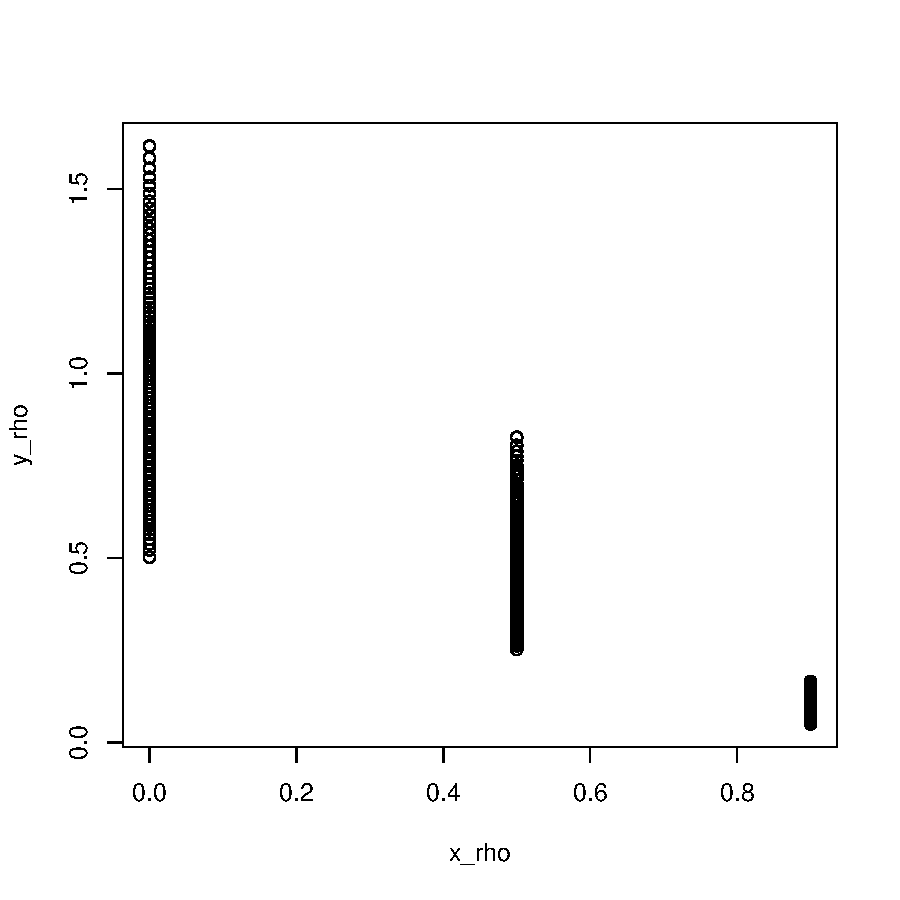
\includegraphics{ps1-plot1}

As $\rho$ moves further away from $0$, we see not just the lowest eigenvalue 
going down (which was the case in (e) already) but the whole set of all eigenvalues 
except the highest one moving towards $0$ (I think the explanation lies
in the joint observation about the highest eigenvalue -- see next paragraph).

Also, interestingly, while all eigenvalues `shrink', the largest one actually blows up. 
Given that the highest eigenvalue (divided by $N$) is the sample variance of 
the first principal component of $\mathbf{X}' \mathbf{X}$, this probably has 
a clear geometric intuition: As the `cloud' of points gets more elongated 
(which reflects high correlation case), there's just one prominent direction of 
very high sample variance that gets `soaked up' by the first component,
leaving variances in the rest of dimensions to be meagre. Oppositely, 
when the cloud is `roundy', there are a lot of different directions in which 
variances are comparable (but not as large as in the high correlation case).

\subsection*{(g)}

\textit{How to read the tables:} Tables -- different choices of $\rho$;
columns -- different sample sizes;
row 1 -- mean $\hat \beta_1$ for $p = 0.9 N$;
row 2 -- variance;
row 3 -- lowest eigenvalues;
row 4, 5, 6 -- the same but for $p = [20 * \log N]$

\textit{Just a random thought}: Is the idea with $20 \cdot \log N$ that if the rate of growth of $p$ is as slow as it's expected to be for lasso to work, then actually OLS doesn't do that much worse? We're not really comparing with lasso here, but at least we see that OLS does the job (probably not as computationally efficiently as lasso?).


This seems to be a weird setting for studying asymptotic properties of estimators
that try to make the model selection concern acute for any possible sample size
($p / N$ not converging to $0$ in contrast to the typical OLS setting). The model is 
equally sparse for any sample size, so it seems like the main determinant of 
the inference properties (how quickly the variance shrinks with the sample size)
is purely the actual number of regressors. In the sense that: we're using
more regressors, so naturally the estimator becomes noisier (depending on
how many regressors the rule prescribes, we get more/less noisier estimates;
and higher covariance just adds noise in the samy way as in (e)).
And we don't gain anything in terms of bias, because there's no additional confounding 
as the sample size increases.

My impression is that in order to meaningfully compare selection regimes 
(to highlight the bias/variance trade-off) we need different DGPs for different 
sample sizes. Actually, this makes me wonder if in the asymptotics for lasso
we keep the set of non-zero coefficients fixed across sample sizes or also
changing? Does the behaviour of the ratio between the number of non-zero and zero
coefficients matter for the properties of lasso? It seems to be a different 
type of condition than the minimum eigenvalue condition. Anyways, the conclusion
I'm making from this part is that if all of the new regressors (that we add
as the sample size increases) are irrelevant in the linear projection of $y$
on all $x$'s, then model selection is also irrelevant.
\begin{Schunk}
\begin{Sinput}
> print(table_g)
\end{Sinput}
\begin{Soutput}
, , 1

            [,1]        [,2]        [,3]        [,4]
[1,] 0.979358646 0.995707198 1.003153285 1.000996911
[2,] 0.109639396 0.054974469 0.019583676 0.010584750
[3,] 0.004177682 0.003490794 0.003072764 0.002896961
[4,] 0.978624749 1.001109901 1.000267763 0.999287602
[5,] 0.139760217 0.010840698 0.002874335 0.001237278
[6,] 0.002810241 0.082050949 0.262248666 0.405071445

, , 2

            [,1]        [,2]        [,3]        [,4]
[1,] 0.980141797 0.984169413 1.006636601 1.002319928
[2,] 0.212526526 0.103930027 0.043846907 0.019755522
[3,] 0.002111150 0.001754069 0.001539565 0.001449988
[4,] 0.981737490 0.998548334 0.999931879 0.999382909
[5,] 0.268858274 0.020893840 0.005561305 0.002289765
[6,] 0.001419683 0.041293406 0.131635124 0.203124413

, , 3

             [,1]         [,2]        [,3]         [,4]
[1,] 0.9802985931 0.9546977569 1.012035088 1.0059677693
[2,] 1.0784679966 0.5176630284 0.221691175 0.0978007126
[3,] 0.0004222941 0.0003508052 0.000307914 0.0002899938
[4,] 0.9840240250 0.9921782195 0.999697018 1.0000302930
[5,] 1.3909375639 0.1074353738 0.026298648 0.0109654547
[6,] 0.0002840300 0.0082617741 0.026328395 0.0406231930
\end{Soutput}
\begin{Sinput}
> 
\end{Sinput}
\end{Schunk}

\end{document}
